% Dette er en del af filerne til eksamensforberedelse til matematik A.
% Copyright (C) 2024 Ricardt Riis
% Se det compilerede dokument for mere information.

\documentclass{article}

\usepackage{amsmath}
\usepackage{amssymb}
\usepackage{amsthm}
\usepackage{graphicx}
\usepackage{float}
\graphicspath{ {./images/} }
\usepackage{pdfpages}
\usepackage{hyperref}
\usepackage[danish]{babel}
\usepackage{tikz}
\usepackage{mathtools}

\usepackage{caption}

\usetikzlibrary {angles, quotes, through}
\usetikzlibrary{calc, tikzmark, intersections}

\usepackage[e]{esvect}

\usepackage{tcolorbox}

\newcommand\gap[0]{\ensuremath{\hspace{1cm}}}

\newcommand\vektor[2]{\ensuremath{
    \begin{pmatrix}
        #1\\
        #2
    \end{pmatrix}
}
}

\newcommand\billede[3][1\textwidth]{\begin{figure}[H]
    \caption{#3}
    \includegraphics[width=#1]{#2}\label{#2}
    \centering
\end{figure}}

\newcommand\cel{\ensuremath{^\circ\mathrm{C}}}
\newcommand\grader{\ensuremath{^\circ}}
\newcommand\dx{\:\mathrm{d}x}
\newcommand\ud{\,\mathrm{d}}

\newcommand\lr{\ensuremath{\Leftrightarrow}}
\newcommand{\R}{\ensuremath{\mathbb{R}}}
\newcommand{\C}{\ensuremath{\mathbb{C}}}
\newcommand\dmht[1]{\frac{\partial}{\partial #1}}

\newcommand\inccounter[1]{\setcounter{#1}{\arabic{#1}+1}}
\newcommand\facit[1]{\underline{\underline{#1}}}

\tcbuselibrary{theorems}

\newcounter{opgave}
\newtcbtheorem[use counter=opgave]{opgave}{Opgave}{separator sign none}{}
\newtcbtheorem[number within=opgave, number format=\alph]{del}{Delopgave}%
{theorem style=plain,colframe=white,coltitle=black,fontupper=\itshape}{}
\newtcbtheorem{formel}{Formel}{theorem style=break,colframe=blue!70!white,coltitle=black!90!white,fonttitle=\itshape}{lm}

\newtcbtheorem[number within=section]{eksempel}{Eksempel}{theorem style=plain, colframe=black, colback=white, %
colbacktitle=blue!30!white,coltitle=black!90!white,fonttitle=\itshape}{ex}
\newtcbtheorem[number within=section]{definition}{Definition}{theorem style=plain, colframe=black, colback=white, boxrule=0.25mm, sharp corners=all,%
colbacktitle=blue!30!white,coltitle=black!90!white,fonttitle=\bfseries}{df}

\newtcbtheorem[number within=section]{theorem}{Sætning}{sharp corners=all, theorem style=plain, colframe=black, colback=white,%
colbacktitle=blue!30!white,coltitle=black!90!white,fonttitle=\bfseries, boxrule=0.25mm}{th}

\newtcbtheorem[number within=section]{lemma}{Lemma}{sharp corners=all, theorem style=plain, colframe=black, colback=white,%
colbacktitle=blue!30!white,coltitle=black!90!white,fonttitle=\bfseries, boxrule=0.25mm}{lm}


\usepackage{makeidx}
\makeindex

%\synctex=1
\newcommand{\Rho}{\mathrm{P}}

\title{Eksamensnoter}
\author{Ricardt Riis}

\newcounter{opgavecnt}
\newcommand{\opg}[1]{\stepcounter{opgavecnt}\textit{Opgave \arabic{opgavecnt}: }#1}

\begin{document}

\maketitle

\begin{quote}
    Copyright \copyright{}  2024  Ricardt Riis.
    Permission is granted to copy, distribute and/or modify this document
    under the terms of the GNU Free Documentation License, Version 1.3
    or any later version published by the Free Software Foundation;
    with no Invariant Sections, no Front-Cover Texts, and no Back-Cover Texts.
    A copy of the license is included in the software \href{https://github.com/Rikibig/exam-prep-math/}{repository}. See also \href{https://www.gnu.org/licenses/fdl-1.3.en.html}{GNU FDL}.
\end{quote}

\textbf{Meningen med materialet er som disposition til mundtlig eksamen}

\tableofcontents

\section*{Introduktion}
I det følgende vil overskriften angive hvilket spørgsmål der svares på. Da det
er bedst at svare på begge spørgsmål "samtidigt" eller i det mindste have en
nogenlunde flydende overgang mellem de to spørgsmål, virker det gavnligst at
beskrive spørgsmålene, og dernæst under \emph{én} overskrift besvare
spørgsmålene.

Der er desuden lagt en række opgaver ind; materialet kan læses uden at løse
opgaverne, men for en dybere forståelse anbefales det at løse dem, som man ikke
umiddelbart kan løse.

\begin{tcolorbox}
    \section{Funktioner}
    \tcblower
    \begin{enumerate}
        \item Giv en præsentation af en selvvalgt del af teorien for vektorfunktioner.
        \item Brug vektorfunktioner til at bestemme de afledte af de trigonometriske funktioner.
    \end{enumerate}
\end{tcolorbox}
Her kan man komme ind på følgende:
\begin{itemize}
    \item Funktioner tager et input, og laver et output.
    \item For vektorfunktioner gælder at deres signatur er
        \[
            \mathbb{R} \rightarrow \mathbb{R}^2.
        \] 
    \item Vektorfunktioner\index{vektorfunktion} skrives
        \[
            \vec{v}(t).
        \] 
    \item $t$ kaldes normalt \texttt{parameterværdi}\index{parameterværdi}.
    \item Præsenteres en vektorfunktion grafisk, benyttes en banekurve\index{banekurve}.\\
        \textit{Bemærk}: En banekurve viser ikke alt ved en vektorfunktion. Fx.
        er banekurverne for $\vektor{t^3}{t^3}$ og $\vektor{t}{t}$ ens.
    \item Den afledede af en vektorfunktion kan bestemmes således
        \[
            \vec{v}\,'(t) = \vektor{x(t)}{y(t)}' = \vektor{x'(t)}{y'(t)}
        \] 
        \textit{I det følgende vil afledte funktioner skrives således}
        \[
            \dot{\vec{v}}(t) = {\vektor{x(t)}{y(t)}}'
        \] 
    \item Den afledede beskriver retningsvektoren for tangenten til en bestemt
        parameterværdi.

    \item Den afledede kaldes også hastighedsvektoren\index{hastighedsvektor}
    \item Dermed kan farten bestemmes ved længden af hastighedsvektoren
        \[
            \text{fart}(\vec{v}) = \left|\dot{\vec{v}}\right|
        \] 
    \item Se mere viden om vektorer i afsnit om vektorer.
\end{itemize}

\begin{definition}{Cosinus, sinus og tangens}{}
    \index{trigonometriske funktioner}
    Cosinus, $\cos$, sinus, $\sin$, og tangens, $\tan$, defineres ud fra
    enhedscirklen\index{enhedscirklen}, der har radius 1.
    \begin{center}
    \begin{tikzpicture}[scale=2.0]
        \coordinate (A) at (0, 0);
        \coordinate (B) at (0.8660254037844387, 0);
        \coordinate (C) at (0.8660254037844387, 0.5);
        \coordinate (E) at (1, 0.5773502691896257);
        \coordinate (D) at (1, 0);
        \draw (A) -- (B) node [midway, below] {$\cos{t}$};
        \draw (C) -- (B) node [midway, left] {$\sin{t}$};
        \draw (A) -> (C) node [midway, above] {$\vec{r}$};
        \draw[dotted, thick] (C) -- (E);
        \draw[dotted, thick] (D) -- (E) node [midway, right] {$\tan{t}$};
        \draw pic [draw] {angle = B--A--C};
        \node [above] at (0.30, -0.025) {$t$};

        \draw[->,thick] (-1.5,0)--(1.5,0) node[right]{$x$};
        \draw[->,thick] (0,-1.5)--(0,1.5) node[above]{$y$};
        \node [draw,circle through=(D)] at (A) {};
    \end{tikzpicture}
    \end{center}
\end{definition}

\opg{Hvilke tal $\phi$ opfylder $\cos(x) = \cos(x + \phi)$?}

\opg{Disse tal fortæller noget om perioden af cosinus. Hvad?}

\opg{Hvilke tal $\phi$ opfylder $\cos(x) = \sin(x + \phi)$?}

\begin{theorem}{Idiotformlen}{idformel}
    \( \cos^2{t} + \sin^2{t} = 1 \)    
\end{theorem}

\opg{Vis sætningen.}

\begin{theorem}{Afledte cosinus og sinus}{cossindiff}
    \begin{align*}
        \cos' &= -\sin\\
        \sin' &= \cos
    \end{align*}
\end{theorem}

\begin{proof}
Lad
\[
    \vec{r}(t) = \vektor{\cos{t}}{\sin{t}}.
\] 
Det ønskes at finde $\dot{\vec{r}}(t)$, da vi i så fald kan bevise sætning
\ref{th:cossindiff}.

\smallskip

Det vides om $\vec{r}$ at den bevæger sig langs enhedscirklens periferi. Dvs.
at for hver omgang $\vec{r}$ bevæger sig omkring periferien, har punktet som
stedvektoren $\vec{r}$ beskriver bevæget sig $2\pi$. Da perioden for $\vec{r}$
også er $2\pi$ ved vi om farten af $\vec{r}$
\[
    |\dot{\vec{r}}(t)| = 1.
\] 
\textit{Bemærk, at længden af $\vec{r}$ også er 1 (jf. sætning \ref{th:idformel}).}\\
Det vides om tangenter til punkter på en cirkel står ret på stedvektoren til
punktet. Dermed gælder
\[
    \dot{\vec{r}} = \hat{\vec{r}}.
\]
Derfor
\begin{align*}
    \dot{\vec{r}} = {\vektor{\cos}{\sin}}' &= \widehat{\vektor{\cos}{\sin}} = \hat{\vec{r}}\\
                        \implies \vektor{\cos'}{\sin'}    &= \vektor{-\sin}{\cos}.
\end{align*}
Da lighedstegnet gælder koordinatvis, er beviset gennemført.
\end{proof}

\opg{Vis at tangenten til et punkt på cirklen står vinkelret på stedvektoren
til punktet.}

\begin{theorem}{Afledede tangens}{difftan}
    \(
        \tan' = \tan^2 + 1
    \) 
\end{theorem}

\begin{proof}
\begin{align*}
    \tan' &= \left(\frac{\sin}{\cos}\right)'\\
          &= \left(\sin \cdot \frac{1}{\cos}\right)'\\
          &= \cos \cdot \frac{1}{\cos} + \sin \cdot \left(\frac{1}{\cos}\right)'\\
          &= 1 + \sin \cdot \left(-\frac{1}{\cos^2}\right) \cdot (-\sin)\\
          &= 1 + \frac{\sin^2}{\cos^2}\\
          &= \tan^2 + 1.\qedhere
\end{align*}
\end{proof}

\opg{Overvej hvorfor tangens er $\frac{\sin}{\cos}$, eller formuleret
anderledes, hvad tangens beskriver.}

\opg{Overvej hvad vektorfunktioner ellers kan bruges til.}

\begin{tcolorbox}
    \section{Funktioner}
    \tcblower
    \begin{enumerate}
        \item Giv en præsentation af en selvvalgt del af teorien for plus- og gangefølger.
        \item Bevis at to gangefølger altid giver anledning til en potenssammenhæng.
    \end{enumerate}
\end{tcolorbox}

\begin{eksempel*}{Hvordan ville jeg gøre?}{}\\
    Jeg ville forklare stoffet i følgende rækkefølge.
    \begin{itemize}
        \item Introducer hvad plusfølger og gangefølger er 
            (definition \ref{df:plusfølge} og \ref{df:gangefølge}).\\
            Gør herunder brug af figur \ref{plus_og_gange} %TODO
        \item Forklar sætning \ref{th:gangegange}, evt. ved brug af figur \ref{gangegange}
        \item Hvis der er mere tid til overs, bevis logaritmeregnereglerne i rækkefølgen
            sætning \ref{th:logswap}, \ref{th:logpotenstilgange} og \ref{th:loggangeplus}.
    \end{itemize}
\end{eksempel*}

\begin{definition}{Logaritme}{log}
    Logaritmen med grundtal $a$ defineres så
    \[
        \log_a{a^x} = x,\qquad a > 0 \text{ og } a \ne 1, x\in\mathbb{R}.
    \] 
\end{definition}

\begin{theorem}{Logaritme laver gange om til plus}{loggangeplus}
    \[\log_A(B \cdot C) = \log_AB + \log_AC\]
\end{theorem}

\begin{proof}
\begin{align*}
    \log_A(B \cdot C) &= \log_AB + \log_AC \iff\\
\intertext{Der opløftes i A for at potensregneregler kan benyttes}
    A^{\log_A(B \cdot C)} &= A^{\log_AB + \log_AC}\\
\intertext{Føromtalte potensregneregel benyttes}
                          &= A^{\log_AB} \cdot A^{\log_AC} \iff\\
\intertext{$A^{\log_A}$ går ud}
    B \cdot C &= B \cdot C\qedhere
\end{align*}
%TODO vend rækkefølgen
\end{proof}

\begin{theorem}{Logaritmeregneregel}{logpotenstilgange}
    $\log_AB^C = C \cdot \log_AB$
\end{theorem}

\begin{proof}
Opløftning er det samme som gentagen gange
\begin{align*}
    \log_AB^C &= \log_A{\underbrace{(B \cdot B \cdots B)}_{C\text{ gange}}}\\
\intertext{Jævnfør sætning \ref{th:loggangeplus}, kan man skrive}
              &= \underbrace{\log_A{B} + \log_A{B} + \cdots + \log_A{B}}_{C\text{ gange}}\\
\intertext{Da der lægges sammen C gange, og gange er gentaget plus, så gælder}
              &= C \cdot \log_AB.\qedhere
\end{align*}
\end{proof}

\textit{Bemærk:} Dette bevis giver dog kun mening for et naturligt $C$, da vi ikke uden videre kan sige hvad det betyder at gange noget med sig selv f.eks. en halv gang.

\opg{Heldigvis er der en udvej. Vis at sætningen ovenfor også gælder for $C \in \mathbb{R}$. \emph{Hint: Benyt at $A^{B \cdot C} = (A^B)^C$}.}

\begin{theorem}{Logaritmeregneregel}{logswap}
    $A^{\log_BC} = C^{\log_BA}$.
\end{theorem}

\begin{proof}
Reglen opskrives
\begin{align*}
    A^{\log_BC} &= C^{\log_BA} \iff\\
\intertext{Vi gør på en smart måde ingenting}
    B^{\log_B{A^{\log_BC}}} &= B^{\log_B{C^{\log_BA}}} \iff\\
\intertext{Ifølge sætning \ref{th:logpotenstilgange} så kan vi}
    B^{\log_BC \cdot \log_B{A}} &= B^{\log_BA \cdot \log_B{C}}\qedhere
\end{align*}
%TODO gør det mere intuitivt.
\end{proof}

\begin{definition}{Plusfølge}{plusfølge}
    En plusfølge lægger altid et bestemt tal til for hvert skridt i følgen.
\end{definition}

\begin{definition}{Gangefølge}{gangefølge}
    En gangefølge gange altid et bestemt tal for hvert skridt i følgen.
\end{definition}

\begin{figure}[H]
    \centering
    \caption{Forklaring af definitionerne}
    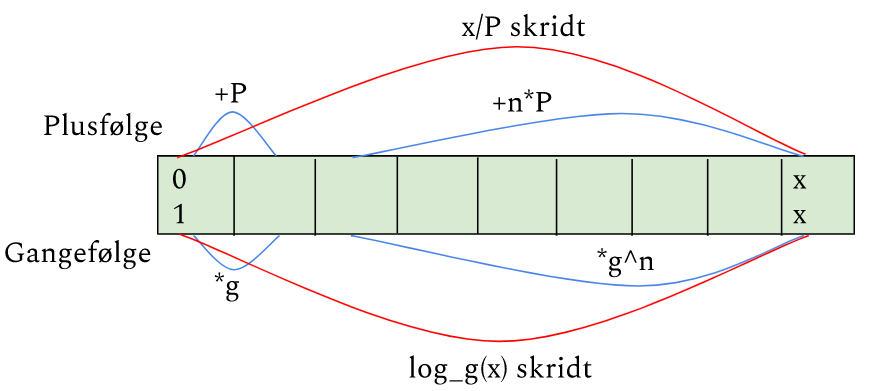
\includegraphics[width=0.8\textwidth]{plus_og_gange}
    \label{plus_og_gange}
\end{figure}

\begin{theorem}{Gangefølge - Gangefølge}{gangegange}
    To gangefølger,
    \begin{center}
        $c\cdot \Rho x^n$ og $d\cdot \Rho y^n$, $c \ne 0 \land \Rho x \ne 0$
    \end{center}
    giver altid anledning til en potenssammenhæng
    \[
        y = \frac{d}{c^{\log_{\Rho x}{\Rho y}}}\cdot x^{\log_{\Rho x}{\Rho y}}.
    \]
    \textit{Bemærk at $c^{\log_{\Rho x}{\Rho y}}$ er 1, hvis x-følgen starter ved 1.}
\end{theorem}

\begin{proof}
$y$ ønskes at kunne blive fundet ud fra vilkårlig $x$. Til det formål skal vi kende
$n$.
\begin{align*}
    x &= c\cdot \Rho x^n\\
    n &= \log_{\Rho x}{\frac{x}{c}}
\end{align*}

Denne $n$ kan indsættes i udtrykket for $y_n$, så enhver $y$ kan findes.
\begin{align*}
    y &= d\cdot \Rho y^{\log_{\Rho x}{\frac{x}{c}}}\\
\intertext{Per sætning \ref{th:logpotenstilgange}}
    &= d\cdot \left(\frac{x}{c}\right)^{\log_{\Rho x}{\Rho y}}\\
\intertext{Potensregneregel}
    &= \frac{d}{c^{\log_{\Rho x}{\Rho y}}}\cdot x^{\log_{\Rho x}{\Rho y}}.\qedhere
\end{align*}
\end{proof}

\begin{figure}[H]
    \centering
    \caption{En grafisk fremstilling af ovenstående}
    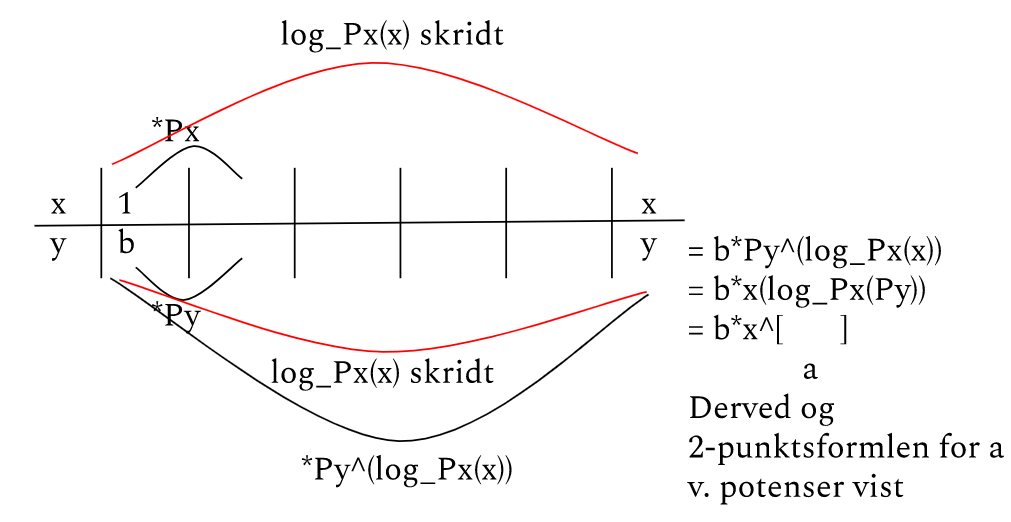
\includegraphics[width=0.8\textwidth]{gangegange}
    \label{gangegange}
\end{figure}

\opg{Overvej hvorfor overvejelser om plus- og gangefølger er interessante.}

\opg{Vis hvordan $y$ kan beskrives i en gange-plusfølge, plus-gangefølge og
plus-plusfølge. \textit{Hint:} Benyt samme idé som i ovenstående bevis.}

\opg{Kan alle følger (ikke nødvendigvis plus- og gangefølger) kombineres med samme idé? \textit{Hint:} Overvej hvis $x$
beskrives ved $n^2$.}

\begin{tcolorbox}
    \section{Funktioner}
    \tcblower
    \begin{enumerate}
        \item Giv en præsentation af en selvvalgt del af teorien for funktioner af to variable.
        \item Udled formlen for hældningen af regressionslinjen ved mindste kvadraters metode.
    \end{enumerate}
\end{tcolorbox}

\begin{eksempel*}{Hvordan ville jeg gøre?}
    Jeg ville
    \begin{enumerate}
        \item Først tale om funktioner (tegne maskinen), og være opmærksom på
            to input.
        \item Tale om definitionen på partiel afledning.
        \item Tale om gradienten og stationære punkter.
        \item Påbegynde beviset for sætning \ref{th:linreg2}, og stoppe ved
            indsigten om
            \[
                \overline{y} = a_{reg} \cdot \overline{x} + b_{reg}.
            \] 
        \item Bevise sætning \ref{th:propreg} og \ref{th:aregpoint}.
        \item Færdiggøre beviset for sætning \ref{th:linreg2}.
    \end{enumerate}
    Derudover ville jeg henlede opmærksomheden på at man også godt kunne bevise
    sætning \ref{th:linreg2} kun ved brug af funktioner af to variable.
\end{eksempel*}

\begin{definition}{Partiel afledning}{pderi}
    En funktion af to variable, $f(x, y)$, kan afledes partielt
    \[
        \frac{\partial}{\partial x} f(x, y) = \lim_{h\rightarrow0} \frac{f(x+h, y) - f(x, y)}{h}.
    \] 
    Der afledes tilsvarende med hensyn til $y$.
\end{definition}

\begin{eksempel*}{Partiel afledning}{}
    Givet funktionen
    \[
        f(x, y) = x^2 + y^3 + xy,
    \] 
    så vil den partielt afledede med hensyn til $x$ være
    \[
        \frac{\partial}{\partial x}f(x, y) = \frac{\partial}{\partial x} x^2 + y^3 + xy = 2x + y.
    \] 
\end{eksempel*}

\opg{Hvad er den afledede med hensyn til $y$?}

\begin{definition}{Gradient}{grad}
    Gradienten til en funktion af to variable, noteret $\nabla$ (nabla), defineres ved
    \[
        \nabla f(x, y) = \vektor{\frac{\partial}{\partial x}f(x, y)}
                           {\frac{\partial}{\partial y}f(x, y)}.
    \] 
\end{definition}

\opg{Bestem $\nabla f(3, 5)$ med samme $f$ som i eksemplet.}

\begin{definition}{Stationære punkter}{station}
    Et stationært punkt til en funktion $f(x, y)$ defineres ved et punkt 
    $(x_0, y_0)$ hvor $x_0$ og $y_0$ opfylder
    \[
        \nabla f(x_0, y_0) = \vec{0} = \vektor{0}{0}.
    \] 
\end{definition}

\begin{definition}{Kvadratsum}{kvsum}
    Givet en funktion $f: \mathbb{R} \to \mathbb{R}$ og $n$ datapunkter på formen
    $(x_i, y_i), x_i, y_i \in \mathbb{R}$, kan kvadratsummen beskrives ved
    \[
        \sum_{i=1}^n (f(x_i) - y_i)^2.
    \] 
\end{definition}

\opg{Overvej hvilken effekt det har, at forskellen mellem forventningen ($f(x_i)$)
og observationen ($y_i$) sættes i anden.}

\begin{theorem}{Proportionalitetsregression}{propreg}
    Den bedste hældning for en ret linje ved brug af mindste kvadraters metode
    gennem (0, 0) er givet ved
    \[
        a_{reg} = \frac{\sum_{i=1}^n x_i \cdot y_i}{\sum_{i=1}^n x_i^2}
    \] 
    hvor $n$ er så mange punkter der laves regression på, og $x_i$ er x-koordinaten
    til det i-te punkt, og $y_i$ tilsvarende er y-koordinaten til det i-te punkt.
\end{theorem}

\begin{proof}
Først opskrives kvadratsummen for en given hældning
\[
    KS(a) = \sum_{i=1}^n (x_i \cdot a - y_i)^2.
\] 

Nu ønskes den optimale hældning $a_{reg}$ fundet, således at kvadratsummen bliver
mindst. Der differentieres og sættes lig nul.
\begin{align*}
    0 &= KS'(a_{reg}) \\
                 &= \left(\sum_{i=1}^n (x_i \cdot a_{reg} - y_i)^2\right)'\\
\intertext{Grundet ledvis differentiation}
                 &= \sum_{i=1}^n \left((x_i \cdot a_{reg} - y_i)^2\right)'\\
                 \intertext{Kædereglen}
                 &= \sum_{i=1}^n \left(2(x_i \cdot a_{reg} - y_i) \cdot x_i\right)\\
                 &= \sum_{i=1}^n \left(2(x_i^2 \cdot a_{reg} - x_i \cdot y_i)\right)\\
                 \intertext{Distributiv lov}
                 &= 2 \cdot \sum_{i=1}^n (x_i^2 \cdot a_{reg} - x_i \cdot y_i)\\
                 \intertext{Da venstresiden er lig nul, divideres med 2}
                 &= \sum_{i=1}^n (x_i^2 \cdot a_{reg} - x_i \cdot y_i)\\
                 \intertext{Kommutativ lov}
                 &= \sum_{i=1}^n x_i^2 \cdot a_{reg} - \sum_{i=1}^n x_i \cdot y_i\\
                 \intertext{Distributiv lov}
                 &= a_{reg} \cdot \sum_{i=1}^n x_i^2 - \sum_{i=1}^n x_i \cdot y_i\\
                 \intertext{$a_{reg}$ isoleres}
         a_{reg} &=  \frac{\sum_{i=1}^n x_i \cdot y_i}{\sum_{i=1}^n x_i^2}.\qedhere
\end{align*}
\end{proof}

\begin{theorem}{Hældning for ret linje gennem givet punkt}{aregpoint}
    Den bedste hældning for en ret linje gennem $(x_0, y_0)$ er givet ved
    \[
        a_{reg} = \frac{\sum_{i=1}^n (x_i-x_0)(y_i-y_0)}{\sum_{i=1}^n (x_i-x_0)^2}
    \] 
    hvor $n$ er så mange punkter der laves regression på, og $x_i$ er x-koordinaten
    til det i-te punkt, og $y_i$ tilsvarende er y-koordinaten til det i-te punkt.
\end{theorem}

\begin{proof}
Koordinatsystemet forskydes således at punktet $(x_0, y_0)$ kommer til at ligge
i origo. Nu kan sætning \ref{th:propreg} benyttes. For at forskyde
koordinatsystemet trækkes $x_0$ fra x-koordinaten for hvert punkt og $y_0$ fra
y-koordinaten for hvert punkt.
\end{proof}

\opg{Hvorfor kan koordinatsystemet forskydes på denne måde?}

\begin{theorem}{Lineær regression}{linreg2}
    Givet en liste af punkter (x, y), så kan man finde den bedste rette linje
    ved mindste kvadraters metode med følgende hældning $a_{reg}$ og
    begyndelsesværdi $b_{reg}$.
    \[
        a_{reg} = \frac{\sum_{i=1}^n (x_i-\overline{y})(y_i-\overline{y})}{\sum_{i=1}^n (x_i-\overline{x})^2}.
    \] 
    \[
        b_{reg} = \overline{y} - a_{reg} \cdot \overline{x}.
    \] 
    hvor $n$ er så mange punkter der laves regression på, og $x_i$ er x-koordinaten
    til det i-te punkt, og $y_i$ tilsvarende er y-koordinaten til det i-te punkt,
    $\overline{x}$ er gennemsnits x-koordinaten og $\overline{y}$ er
    gennemsnits y-koordinaten.
\end{theorem}

\begin{proof}
Kvadratsummen for den lineære regression opskrives
\[
    KS(a, b) = \sum_{i=1}^n (x_i \cdot a + b - y_i)^2.
\] 
Da det ønskes at finde minimum for funktionen, og et minimum er et stationært
punkt, og der kun er et stationært punkt for funktionen, som også er et
minimum, kan definition \ref{df:station} bruges.

\opg{Hvorfor er der kun et stationært punkt, som er et minimum? \emph{Hint: Betragt evt. graden af de partielt afledede.}}

\smallskip

If. definition \ref{df:grad}
\[
    \frac{\partial}{\partial a} KS(a_{reg}, b_{reg}) = 0 \: \land \:
    \frac{\partial}{\partial b} KS(a_{reg}, b_{reg}) = 0.
\] 
Ligningssystemet løses, først afledes kvadratsumsfunktion med hensyn til
begyndelsesværdien.
\begin{align*}
    0 &= \frac{\partial}{\partial b} KS(a_{reg}, b_{reg})\\
      &= \frac{\partial}{\partial b} \sum_{i=1}^n (x_i \cdot a_{reg} + b_{reg} - y_i)^2\\
      &= \sum_{i=1}^n 2 \cdot (x_i \cdot a_{reg} + b_{reg} - y_i)\\
      &= 2 \cdot \sum_{i=1}^n (x_i \cdot a_{reg} + b_{reg} - y_i)\\
      &= n \cdot b_{reg} + \sum_{i=1}^n (x_i \cdot a_{reg} - y_i)\\
      &= b_{reg} + \sum_{i=1}^n (\frac{x_i}{n} \cdot a_{reg} - \frac{y_i}{n})\\
      \intertext{Det indføres, at $\overline{x} = \sum_{i=1}^n \frac{x_i}{n}$.
          \opg{Overvej hvad $\overline{x}$ betyder.}}
      &= b_{reg} + (\overline{x} \cdot a_{reg} - \overline{y})\\
      \intertext{Nu kan enten $a$ eller $b$ isoleres, og der kan differentieres
          partielt med hensyn til den anden variabel, ligningssystemet kan
      løses. I stedet indses følgende}
    \overline{y} &= a_{reg} \cdot \overline{x} + b_{reg}
\end{align*}
Dette er meget centralt, for det fortæller, at punktet $\overline{x}$ og
$\overline{y}$ ligger på regressionslinjen. Dermed kan hældningen findes ved
sætning \ref{th:aregpoint}
\[
    a_{reg} = \frac{\sum_{i=1}^n (x_i-\overline{y})(y_i-\overline{y})}{\sum_{i=1}^n (x_i-\overline{x})^2}.
\] 
Begyndelsesværdien er triviel at finde
\[
    b_{reg} = \overline{y} - a_{reg} \cdot \overline{x}.\qedhere
\] 
\end{proof}

\opg{Fortsæt beviset uden brug af smarte indsigter ved at aflede mht. $a_{reg}$
og løse det efterfølgende ligningssystem.}

\opg{Overvej hvor man bruger lineær regression.}

\opg{Overvej hvilke konsekvenser det har, at regressionen bruger minste
kvadraters metode.}

\begin{tcolorbox}
    \section{Differential- og integralregning}
    \tcblower
    \begin{enumerate}
        \item Giv en præsentation af en selvvalgt del af teorien for diskret analyse.
        \item Bevis mindst en regneregel for diskret differentiation.
    \end{enumerate}
\end{tcolorbox}
\begin{itemize}
    \item I diskret analyse benyttes talfølger; i stedet for talfunktioner.
    \item For at gøre notationen af uendeligt lange talfølger nemmere, kan man benytte sig af funktionsnotation
        \[
            f(x), x\in\mathbb{N}.
        \]
        \begin{eksempel}{Indeksering}{}\\
            Hvis $f$ defineres ved talfølgen $1, 3, 5, 4, 9$, så vil
            \[
                f(3) = 5,
            \] 
            og $f(2.5)$ være udefineret.
        \end{eksempel}
    \item Der indføres desuden en anden potensfunktion
        \[
            x^{\overline{n}} = \frac{x!}{(x-n)!}
        \] 
        \begin{eksempel}{x i n-streg}{x-i-n-streg}
            $
                7^{\overline{4}} = 7 \cdot 6 \cdot 5 \cdot 4.
            $ 
        \end{eksempel}
        \opg{Beregn $6^{\overline{3}}$.}
    \item Det kaldes at differentiere når man trækker nabo-elementer fra hinanden
        \[
            \Delta f: [2, 2, -1, 5].
        \] 
    \item Det kan skrives med symboler
        \begin{definition}{Differentiation}{diff}
            $
                \Delta f(x) = f(x + 1) - f(x).
            $ 
        \end{definition}
    \item Man kan desuden definere integration
        \begin{definition}{Integration}{dint}
            Givet en talfølge defineret ved alle heltal i intervallet 
            $[a;b],\: a,b\in\mathbb{Z}$, så er alle stamfølger givet ved
            \[
                F(x_0) = \sum_a^{x_0} f(x) + k,
            \]
            hvor $k \in \mathbb{R}$.
        \end{definition}
    \item Det følger let at følgende gælder
        \begin{theorem}{Integralregningens hovedsætning}{main}
            \[
                \sum_a^b f(x) = F(b + 1) - F(a)
            \]
        \end{theorem}
        \opg{Vis integralregningens hovedsætning for følger. \textit{Hint:}
        Brug defintion \ref{df:dint}.}
\end{itemize}

\begin{definition}{Produkt af to følger}{listproduct}
    $ (f \cdot g)(x) = f(x) \cdot g(x) $
\end{definition}

\begin{theorem}{Produktregel for differentiation}{produktdiff}
    \[
        \Delta (f \cdot g)(x) = \Delta f(x) \cdot g(x) + f(x + 1) \cdot \Delta g(x)
    \] 
\end{theorem}

\begin{proof}
\begin{align*}
    \Delta (f \cdot g)(x) &= \Delta (f(x) \cdot g(x))\\
    \intertext{Ud fra definition af at gange to følger med hinanden}
                          &= f(x + 1) \cdot g(x + 1) - f(x) \cdot g(x)\\
                          &= f(x + 1) \cdot (g(x) + \Delta g(x)) - (f(x + 1) - \Delta f(x)) \cdot g(x)\\
                          &= f(x + 1) \cdot g(x) + f(x + 1) \cdot \Delta g(x) \\
                          &\gap- f(x + 1) \cdot g(x) + \Delta f(x) \cdot g(x)\\
                          &= \tcbhighmath{f(x + 1) \cdot g(x)} + f(x + 1) \cdot \Delta g(x) \\
                          &\gap\tcbhighmath{- f(x + 1) \cdot g(x)} + \Delta f(x) \cdot g(x)\\
                          &= f(x + 1) \cdot \Delta g(x) + \Delta f(x) \cdot g(x)\qedhere
\end{align*}
\end{proof}

\opg{Undersøg hvad der sker, hvis skridtlængden går mod 0.}

\begin{theorem}{Differentiation af $x^{\overline{n}}$}{diffxn}
    Givet konstant $n$ og variabel $x$ gælder
    \[
        \Delta x^{\overline{n}} = n \cdot x^{\overline{n-1}}.
    \]
\end{theorem}
\begin{proof}
\begin{align*}
    \Delta x^{\overline{n}} &= (x+1)^{\overline{n}} - x^{\overline{n}}\\
    &= (x+1) \cdot x^{\overline{n-1}} - x^{\overline{n-1}} \cdot (x - (n-1))\\
    &= (x + 1 - x + (n - 1)) \cdot x^{\overline{n-1}}\\
    &= n \cdot x^{\overline{n-1}}.\qedhere
\end{align*}
\end{proof}

\opg{Overvej hvorfor den sidste faktor er $(x - (n-1))$. \textit{Hint:} Se
eksempel \ref{ex:x-i-n-streg}.}

\begin{tcolorbox}
    \section{Differential- og integralregning}
    \tcblower
    \begin{enumerate}
        \item Giv en præsentation af en selvvalgt del af teorien for
            differential- og integralregning        
        \item Bevis mindst en regneregel for differentiation    
    \end{enumerate}
\end{tcolorbox}

\begin{eksempel*}{Hvordan ville jeg gøre?}
    \begin{enumerate}
        \item Bevise sætning \ref{th:chainrule}, inddrage viden om kontinuitet
            og differentiabilitet,
        \item Bevise sætning \ref{th:xinte} ved brug af sætning
            \ref{th:difflog} og \ref{th:chainrule}
        \item Bevise sætning \ref{th:difflog}
    \end{enumerate}
\end{eksempel*}

I disse noter er der en forhåbning om at læseren har en intuition for hvad en
grænseværdi er, thi definitionen er noget bøvlet.

\begin{definition}{Kontinuitet}{kont}
    Hvis grænseværdien for $f(x)$ når $x$ går mod $x_0$ er $f(x_0)$
    \[\lim_{x\to x_0} f(x) = f(x_0),\]
    så er $f$ kontinuert.
\end{definition}

For at noget skal være kontinuert, skal, hvis $x$-værdierne er tæt på hinanden,
$y$-værdierne også være tæt på hinanden. Vi går ud fra, at alle
standardfunktioner er kontinuerte.

\opg{\textit{Temmelig svær, i væsentlig grad uden for pensum}, Vis at
standardfunktionerne er kontinuerte. Det tager kun et semester på uni.}

\newcommand\sek[2]{d_{#1,#2}}
\begin{definition}{Sekanthældning}{sekant}
    Sekanthældningen er hældningen for en ret linje gennem to forskellige
    punkter på en funktion $f$,
    \[
        d_{f,x_0}(x) = \frac{f(x) - f(x_0)}{x - x_0}.
    \] 
\end{definition}

\begin{definition}{Differentiabilitet}{diffhed}
    Differentialkvotienten er grænseværdien for sekanthældningen for $f$ i
    x-værdierne $x$ og $x_0$ når $x$ går mod $x_0$
    \[f'(x_0) = \lim_{x \to x_0} d_f(x)\]
\end{definition}

\opg{Hvorfor er funktionen $f(x) = |x|$ kontinuert i $x = 0$, men ikke differentiabel?}

\begin{theorem}{Kædereglen}{chainrule}
    \[
        (f \circ g)' = (f' \circ g) \cdot g'
    \] 
\end{theorem}

\begin{proof}
\begin{align*}
    d_{f \circ g,x_0}(x) &= \frac{(f \circ g)(x) - (f \circ g)(x_0)}{x - x_0}\\
                      &= \frac{f(g(x)) - f(g(x_0))}{x - x_0}\\
    \intertext{Der ganges med 1 på en sjov måde}
                      &= \frac{f(g(x)) - f(g(x_0))}{x - x_0} \cdot 
                      \frac{g(x) - g(x_0)}{g(x) - g(x_0)}\\
    \intertext{Vha. brøkregneregel}
                      &= \frac{f(g(x)) - f(g(x_0))}{g(x) - g(x_0)} \cdot 
                      \frac{g(x) - g(x_0)}{x - x_0}\\
                      &= d_{f,g(x_0)}(g(x)) \cdot d_{g,x_0}(x)
\end{align*}
Grundet viden om sekanthældninger og grænseværdier
\begin{align*}
    \lim_{x \to x_0} d_{f \circ g,x_0}(x) &= (f \circ g)'(x_0)\\
             &= \lim_{x \to x_0} d_{f,g(x_0)}(g(x)) \cdot d_{g,x_0}(x)\\
    \intertext{Når $x$ går mod $x_0$, og hvis $g$ er kontinuert og ikke
    konstant, så går $g(x)$ mod $g(x_0)$. Dermed}
             &= f'(g(x_0)) \cdot g'(x_0)
\end{align*}
Da $x_0$ er vilkårlig gælder
\[
    (f \circ g)' = (f' \circ g) \cdot g'.\qedhere
\] 
\end{proof}

\opg{Afled $e^{5x^2}$.}

\opg{Overvej hvad der sker hvis $g$ er konstant.}

\begin{theorem}{Afledte logaritme}{difflog}
    $(\ln \cdot)' = \frac{1}{\cdot}$
\end{theorem}

\begin{proof}
Med kædereglen
\begin{align*}
    e^{\ln x} &= x\\
    \left( e^{\ln x} \right)' &= x'\\
    x \cdot (\ln x)' &= 1\\
    (\ln x)' &= \frac{1}{x}
\end{align*}
Da $x$ er vilkårlig
\[
    (\ln \cdot )' = \frac{1}{\cdot}.\qedhere
\] 
\end{proof}

\begin{theorem}{Afledte $\cdot^{n}$}{xinte}
    \[
        (\cdot^n)' = n \cdot ^{n-1}
    \] 
\end{theorem}

\begin{proof}
Lad $x \in \mathbb{R}$. Så er
\begin{align*}
    (\ln{x^n})' &= (n \cdot \ln{x})'\\
    (\ln{x^n})' &= n (\ln{x})'\\
    \frac{1}{x^n} \cdot (x^n)'    &= n \cdot \frac{1}{x}\\
    (x^n)' &= x^n \cdot n \cdot \frac{1}{x}\\
           &= n \cdot x^{n-1}
\end{align*}
Og da $x$ er vilkårlig
\[
    (\cdot^n)' = n \cdot ^{n-1}.\qedhere
\] 
\end{proof}

\opg{Hvorfor er det vigtigt at foretage det sidste skridt i beviserne?}

\opg{Hvad kan differentialregningen bruges til?}

\begin{tcolorbox}
    \section{Differential- og integralregning}
    \textbf{Dette afsnit er ufærdigt og upålideligt. Der er mindst en fejl i
    afsnittet. Hvis man ønsker, så kan man jo prøve at finde den.}
    Ellers kan man håbe der på et tidspunkt kommer en opdateret udgave på \href{https://github.com/Rikibig/exam-prep-math}{github.com/Rikibig/exam-prep-math}.
    \tcblower
    \begin{enumerate}
        \item Giv en præsentation af en selvvalgt del af teorien for 
            differential- og integralregning
        \item Redegør for sammenhængen mellem stamfunktion og areal
    \end{enumerate}
\end{tcolorbox}
Se definitioner i tidligere afsnit.

\begin{theorem}{Stamfunktion}{stamfn}
    Lad $f$ være en kontinuert funktion defineret i intervallet $[a; b]$. Da er
    $f$s stamfunktion, $F$,
    \[
        F(x) = \int_a^x f(t) \dx,\quad x \leq b.        
    \] 
\end{theorem}
% TODO: jeg er noget forvirret, for jeg ser hvad wikipedia mener, men vi har i
% klassen fået præsenteret det geometriske forståelse... Hvordan viser man
% dette bedst?

\begin{proof}
% TODO: forklar bedre, indsæt figur.
Antag, at $A(x)$ måler "arealet" under en graf fra $-\infty$ til $x$. Arealet
har her et fortegn, dvs. at hvis grafen er under nul, så tæller den negativt,
medens hvis grafen er over nul så tæller den positivt.

Ønsker man at finde arealet mellem to x-koordinater $x$ og $x_0$, kan dette
lade sig gøre ved
\[
    A(x) - A(x_0).
\] 
Dette udtryk kan approximeres, men der kommer en fejl, kaldet $E$
\[
    A(x) - A(x_0) = f(x_0) \cdot (x-x_0) + E.
\] 

\opg{Overvej hvad approximationen giver står til udtryk for.}\\
Der divideres med $x-x_0$.
\begin{align*}
    \frac{A(x)-A(x_0)}{x-x_0} &= f(x_0) + \frac{E}{x-x_0}\iff\\
    \sek{A}{x_0}(x) &= f(x_0) + \frac{E}{x-x_0} \xlongrightarrow[x \to x_0]{}\\
    A'(x_0) &= \lim_{x \to x_0} f(x_0) + \frac{E}{x-x_0}
\end{align*}

Det undersøges nu, hvad der sker med $\frac{E}{x-x_0}$, når $x \to x_0$.
Vi ved om $E$
\[
    E \le (f(x_h) - f(x_l))(x-x_0),
\] 
hvor $x_h$ og $x_l$ noterer x-koordinaten til henholdsvis det højeste og
laveste punkt på grafen mellem $x$ og $x_0$. Men fordi $x_h$ og $x_l$ skal
ligge mellem $x$ og $x_0$, så vil både $x_h$ og $x_l$ gå mod $x_0$ når $x$ går
mod $x_0$. Med lidt omskrivninger og klemmelemmaet fås altså
\begin{align*}
    \frac{E}{x-x_0} &\le f(x_h) - f(x_l) \xlongrightarrow[x \to x_0]{}\\
                    &= f(x_0) - f(x_0)\\
                    &= 0.
\end{align*}
Dvs.
\begin{align*}
    A'(x_0) &= \lim_{x \to x_0} f(x_0) + \frac{E}{x-x_0}\\
           &= f(x_0) + 0,
\end{align*}
fordi $f(x_0)$ ikke påvirkes af $x$. Altså er $A$ en stamfunktion til $f$.
\end{proof}

\begin{theorem}{Integralregningens hovedsætning}{mainruleint}
    Givet en funktion $f$ der er kontinuert
    \[
        \int_a^b f(x) \dx = F(b) - F(a),
    \]
    hvor $F$ er en stamfunktion til $f$.
\end{theorem}

\opg{(joke) Vis ovenstående sætning.}

\begin{tcolorbox}
    \section{Differensligninger}
    \tcblower
    \begin{enumerate}
        \item Giv en præsentation af en selvvalgt del af teorien for differensligninger.
        \item Udled en løsningsformel til en selvvalgt type differensligning
    \end{enumerate}
\end{tcolorbox}

\begin{theorem}{Sum af potenser}{sumpot}
    \[
        \sum_{x=a}^b g^x = \frac{g^{b+1} - g^a}{g-1}.
    \] 
\end{theorem}

\begin{proof}
$g^x$ er en følge der integreres, ganske som i diskret analyse. Dermed skal der
blot findes en stamfølg til $g^x$. Det er $\frac{1}{g-1} g^x$.

\opg{Vis at $\frac{1}{g-1}g^x$ er en stamfølge til $g^x$.}

\medskip

Således gælder
\begin{align*}
    \sum_{x=a}^b g^x &= \frac{1}{g-1} g^{b+1} - \frac{1}{g-1} g^a\\
                     &= \frac{g^{b+1} - g^a}{g-1}.\qedhere
\end{align*}
\end{proof}


\begin{theorem}{Løsningsformel for $\Delta f(x) = r \cdot f(x) + p$}{differensligningen}
    \[
        \Delta f(x) = r\cdot  f(x)+p, f(0) = b 
        \implies f(x) = b \cdot (r + 1)^x + p \cdot \frac{(r+1)^x - 1}{r},
    \] 
    hvor $p, b \in \mathbb{R}$ og $r \ne 0$.
\end{theorem}

\begin{proof}
Der defineres følgende for at undgå skrivekrampe $g = r+1$.

\smallskip

Første 4 elementer i $f$ skrives op.
\begin{align*}
    f(0) &= b\\
    f(1) &= g \cdot b + p\\
    f(2) &= g^2 \cdot b + gp + p\\
    f(3) &= g^3 \cdot b + g^2p + gp + p
\end{align*}
Det indses dermed hurtigt at følgende gælder
\[
    f(x) = g^x \cdot b + \sum_{i=0}^{x-1} g^i \cdot p
\] 
Efter en omskrivning
\[
    f(x) = b \cdot g^x + p \cdot \sum_{i=0}^{x-1} g^i
\] 

\opg{Forklar omskrivningen}

Grundet sætning \ref{th:sumpot}
\begin{align*}
    f(x) &= b \cdot g^x + p \cdot \frac{g^x - 1}{g - 1} \\
    &= b \cdot (r + 1)^x + p \cdot \frac{(r+1)^x - 1}{r}.\qedhere
\end{align*}
\end{proof}

\opg{Hvad kan man bruge denne differensligning til?}

\bigskip

%\newcommand\vbinom[2]{\ensuremath{\binom{#1}{#2}}} % I fald man kan lide "almen" notation.
\newcommand\vbinom[2]{\ensuremath{\nobreak{K(#1,\,#2)}}} % I fald man ikke kan ...
\begin{tcolorbox}
    \section{Sandsynlighedsregning}
    \tcblower
    \begin{enumerate}
        \item Giv en præsentation af selvvalgt del af teorien for
            sandsynlighedsregning med fokus på binomialfordelingen.
        \item Bevis formlen $\vbinom{n}{r} = \frac{n^{\overline{r}}}{r!}$ ved at løse
            differensligningen \[\vbinom{n+1}{r} = \vbinom{n}{r-1} + \vbinom{n}{r}.\]
    \end{enumerate}
\end{tcolorbox}

\opg{(Svær) Bevis differensligningens gyldighed ved at tælle på to måder.}
\smallskip

\begin{theorem}{Binomialkoefficient}{binkoeff}
    Givet to ikke negative hele tal, $n$ og $r$, hvor $r \le n$ gælder det at
    binomialkoefficienten $\vbinom{n}{r}$ er på formen
    \[
        \vbinom{n}{r} = \frac{n^{\overline{r}}}{r!}.
    \] 
    \vbinom{n}{r} udtales "\textit{n} vælg \textit{r}", og skrives tit
    $\binom{n}{r}$.
\end{theorem}

\begin{proof}
Følgende differensligning indføres
\[
    \vbinom{n+1}{r} = \vbinom{n}{r-1} + \vbinom{n}{r}.
\] 

Det viser sig at være smart at isolere \vbinom{n}{r-1}.
\begin{align*}
    \vbinom{n}{r-1} &= \vbinom{n+1}{r} - \vbinom{n}{r}\\
    \intertext{\vbinom{n}{r} kaldes for det $n$'te element i den $r$'te følge}
    f_{r-1}(n) &= f_{r}(n+1) - f_{r}(n)\\
    \intertext{Idé fra diskret analyse indføres}
    f_{r-1}(n) &= \Delta f_{r}(n)
\end{align*}

Det er et super centralt resultat, for nu kan alle $f_{r}$ findes. Det skyldes
at $f_0(n)$ er kendt, og en hvilken som helst $f_r(n)$ kan findes ved at
integrere diskret $r$ gange med pluskonstant 0, og evaluere i $n$. Bevis ved
induktion.

\smallskip

\textbf{Startbetingelse:} $f_0(n) = 1$, da \vbinom{n}{0} er 1, fordi der kun kan
vælges nul elementer på en måde.

\textbf{Induktionsskridt:} Under antagelse af at $f_r(n) =
\frac{n^{\overline{r}}}{r!}$, vis da at $f_{r+1}(n)
=\frac{n^{\overline{r+1}}}{(r+1)!}$.

Idéen fra diskret analyse bruges nu
\begin{align*}
    f_{r}(n) 
       &= \frac{n^{\overline{r}}}{r!}\\
       &= \frac{(r+1) \cdot n^{\overline{r}}}{(r+1)!}\\
       &= \frac{\Delta n^{\overline{r+1}}}{(r+1)!}\\
       &= \Delta\frac{n^{\overline{r+1}}}{(r+1)!}\\
       &= \Delta f_{r+1}(n)
\end{align*}
Det vil sige
\begin{align*}
    \Delta f_{r+1}(n) &= \Delta\frac{n^{\overline{r+1}}}{(r+1)!}\\
    f_{r+1}(n) &= \frac{n^{\overline{r+1}}}{(r+1)!}
\end{align*}
Dermed er induktionsbeviset afsluttet.

\smallskip

Da det nu er vist at $f_r(n) = \frac{n^{\overline{r}}}{r!}$, og $f_r(n) =
\vbinom{n}{r}$, da er differensligningen løst.
\end{proof}

\opg{($\neg$pensum) Overvej hvorfor et induktionsbevis er gyldigt.}

\begin{definition}{Tæthedsfunktion}{thickfunc}
    En funktion $f$ defineret i udfaldsmængden for en stokastisk variabel $X$ givet
    ved mængden $\Omega$ er en tæthedsfunktion hvis og kun hvis den opfylder
    \[
        f(x) \ge 0, \forall x \in \Omega \qquad \text{og} \qquad \int_\Omega f(x) \dx = 1.
    \] 
    Tæthedsfunktionen angiver sandsynligheden for et givent udfald
    \[
        P(X=x) = f(x).
    \] 
\end{definition}

\begin{definition}{Bernoullifordeling}{bern}
    En bernoullifordelt stokastisk variabel har tæthedsfunktionen
    \[
        f(x) = 
        \begin{cases} 
            p & x = 1\\
            (1 - p) & x = 0
        \end{cases}
    .\] 
\end{definition}

\opg{Hvorfor er ovenstående en tæthedsfunktion?}

\smallskip

\begin{theorem}{Binomialfordelingen}{binomford}
    %TODO Sandsynlighed for succes?
    Givet $n$ bernoullifordelte stokastiske variable, $X$, med sandsynlighed
    for succes $p$, defineres en binomialfordelt stokastisk variabel som
    \[
        Y = \sum_{i=1}^{n} X_i
    ,\] 
    eller bare
    \[
        Y \sim bin(n, p).
    \] 
    Så gælder
    \[
        P(Y = r) = p^r \cdot (1 - p)^{n-r} \cdot \vbinom{n}{r}.
    \] 
\end{theorem}

\begin{proof}
Hvis en bernoullifordelt stokastisk variabel er lig med 1, kaldes udfaldet for
en succes, $s$, ellers fiasko, $f$. For at spare på blækket skrives
$P(s\:\text{og}\:f)$ som $P(sf)$. Således fås
\begin{align*}
    P(Y = r) &= P(\underbrace{ss \dotso s}_r \underbrace{ff \dotso f}_{n-r})\\ 
             &+ P(\underbrace{ss \dotso s}_{r-1} \underbrace{ff \dotso f}_{n-r}s)\\
             &+ P(\underbrace{ss \dotso s}_{r-2} \underbrace{ff \dotso f}_{n-r}ss)\\
             &+ \dotsb
\end{align*}
hvor summeringen forsætter med andre permutationer af $r$ successer og $(n-r)$
fiaskoer. Det viser sig, at alle disse permutationer er ens, som følge af
multiplikationsprincippet og den kommutative lov for gange. Dvs.
\begin{align*}
    P(Y = r) &= P(\underbrace{ss \dotso s}_r \underbrace{ff \dotso f}_{n-r}) \cdot \text{værdi}.\\
    \intertext{Herfra kan sandsynligheden beregnes}
             &= \underbrace{P(s) \cdot P(s) \dotsm P(s)}_r \cdot 
             \underbrace{P(f) \cdot P(f) \dotsm P(f)}_{n-r} \cdot \text{værdi}\\
             &= P(s)^r \cdot P(f)^{n-r} \cdot \text{værdi}\\
             &= p^r \cdot (1-p)^{n-r} \cdot \text{værdi}.
\end{align*}


Nu mangles det blot at finde hvor mange forskellige permutationer der er. For at
finde det, kan man forestille sig at man blandt de $n$ bernoullifordelte
stokastiske variable, så vælges $r$ af dem til at være successer. Dette kan, per
vores binomialkoefficient gøres på netop \vbinom{n}{r} måder. Altså fås
\[
    P(Y = r) = p^r \cdot (1-p)^{n-r} \cdot \vbinom{n}{r}.\qedhere
\] 
\end{proof}

\begin{tcolorbox}
    \section{Statistik}
    \tcblower
    \begin{enumerate}
        \item Giv en præsentation af en selvvalgt del af teorien for
            hypotesetest.
        \item Bevis formlen for 95\%-konfidensintervallet for populationens
            sandsynlighedsparameter ud fra stikprøveandelen.     
    \end{enumerate}
\end{tcolorbox}

\begin{itemize}
    \item Nulhypotese
    \item Hvornår er hvad rigtigt?
    \item Bevis
        \[
            P(p\in[\hat p \pm 2\cdot\sqrt{\frac{\hat p\cdot(1-\hat p)}{n}}]) \approx 95\%
        \]
\end{itemize}

\begin{theorem}{95\%-konfidensinterval}{95konfidens}
    Lad $X$ være en bernoullifordelt stokastisk variabel med
    sandsynlighedsparameter $p$. Givet en stikprøveandel $\hat{p}$ givet ved
    $\frac{1}{n}\sum_{i=1}^n X_i$ kan der opstilles et 95\% konfidensinterval
    for sandsynlighedsparameteren:
    \[
        P\left(p\in\left[\hat p \pm 2\cdot\sqrt{\frac{\hat p\cdot(1-\hat p)}{n}}\right]\right)
        \approx 95\%.
    \] 
\end{theorem}

\begin{proof}
    Antag $p$ er kendt. Da er det muligt at finde et 95\%-konfidensinterval for
    $\hat{p}$
    \[
        P\left(\hat{p}\in\left[p \pm 2\cdot\sqrt{\frac{p\cdot(1-p)}{n}}\right]\right)
        \approx 95\%.
    \] 
    Sandsynligheden for at en stikprøveandel $\hat{p}$ optræder ved
    sandsynlighedsparameter $p$ er den samme som at $p$ optræder som
    stikprøveandel ved sandsynlighedsparameter $\hat{p}$. Derfor kan der i
    konfidensintervallet byttes om på $p$ og $\hat{p}$
    \[
        P\left(p\in\left[\hat p \pm 2\cdot\sqrt{\frac{\hat p\cdot(1-\hat p)}{n}}\right]\right)
        \approx 95\%.\qedhere
    \]
\end{proof}

\begin{tcolorbox}
    \section{Transformationer}
    \tcblower
    \begin{enumerate}
        \item Giv en præsentation af en selvvalgt del af teorien for transformation af funktioner.
        \item Udled forskriften for tæthedsfunktionen for normalfordelingen. 
    \end{enumerate}
\end{tcolorbox}

Man kan flytte funktioner op og ned og hid og did. Hertil kan man justere på
følgende konstanter
\[
    f(x - d) + c.
\] 
Efter en sådan transformation, er $f$ flyttet $d$ til højre og $c$ op. Bemærk
at både $d$ og $c$ kan være negative.

\smallskip

\opg{Vis at ovenstående formodning passer.}

\smallskip

Derudover kan funktioner strækkes
\[
    a \cdot f(\frac{x}{b}),
\] 
hvor $a$ angiver lodret stræk, og $b$ horizontalt.

\begin{theorem}{Om stræk}{straek}
    Givet en funktion $f$ som opfylder
    \[
        \int_{-\infty}^{\infty} f(x) \ud x = k,
    \] 
    hvor $k$ er endelig, gælder det, at en hvis en funktion strækkes med $a$
    lodret, så bliver integralet tilsvarende $a$ større, og hvis en funktion
    strækkes med $b$ vandret, så bliver integralet også $b$ gange større.
\end{theorem}

\begin{proof}[Bevis for vandret stræk]
    Lad en funktion $f$ opfylde
    \[
        \int_{-\infty}^{\infty} f(x) \ud x = k,
    \] 
    hvor $k$ er endelig. Efter et stræk er integralet givet ved
    \[
        \int_{-\infty}^{\infty} f\left(\frac{x}{b}\right) \ud x.
    \] 
    For at kunne bestemme integralet skal der findes en stamfunktion til
    $f(\frac{x}{b})$. Man finder at følgende er en stamfunktion
    \[
        b \cdot F(\frac{x}{b}).
    \] 
    Jf. integralregningens hovedsætning
    \begin{align*}
        \int_{-\infty}^{\infty} f\left(\frac{x}{b}\right) \ud x &= \left[b \cdot F\left(\frac{x}{b}\right) \right]_{-\infty}^{\infty}\\
            &= b \cdot \left[F\left(\frac{x}{b}\right) \right]_{-\infty}^{\infty}\\
            &= b \cdot k.\qedhere
    \end{align*}
\end{proof}

\opg{Bevis resten af sætningen.}

\opg{Overvej om der er et stærkere resultat.}

\begin{definition}{Klokkekurve}{clock}
    Klokkekurven er det første skridt mod normalfordelingen
    \[
        e^{-\frac{1}{2}x^2}.
    \] 
\end{definition}

Vi ønsker at lave klokkekurven om til en tæthedsfunktion, jf. definition
\ref{df:thickfunc}. Den skal altså opfylde at være positiv alle vegne, og at
arealet under grafen er 1.

\opg{Vis at første del af kravet er opfyldt.}

\smallskip

For at gøre arealet under grafen til 1, må der altså strækkes lodret med den
multiplikativt inverse til arealet under klokkekurven. Derfor vises følgende
sætning.

\begin{theorem}{Integral af klokkekurven}{intklokke}
    \[
        \int_{-\infty}^\infty e^{-\frac{1}{2} x^2} \ud x = \sqrt{2 \cdot \pi}.
    \] 
\end{theorem}
\begin{proof}
    Det viser sig at være umådeligt svært at finde en stamfunktion til
    klokkefunktionen. I stedet sættes integralet i anden, og vi ser hvad der
    sker
    \begin{align*}
        \left(\int_{-\infty}^\infty e^{-\frac{1}{2} x^2} \ud x\right)^2 &= \int_{-\infty}^\infty e^{-\frac{1}{2} x^2} \ud x \cdot \int_{-\infty}^\infty e^{-\frac{1}{2} x^2} \ud x\\
        \intertext{Vi vælger lige at kalde den ene variabel $y$.}
         &= \int_{-\infty}^\infty e^{-\frac{1}{2} x^2} \ud x \cdot \int_{-\infty}^\infty e^{-\frac{1}{2} y^2} \ud y\\
         \intertext{Det er klart at integralet der afhænger af $y$ ikke
             afhænger af $x$, og dermed er en gangekonstant. Altså bruges den
         distributive lov\footnote{Ikke helt... men hvorfor?}.} % TODO
         &= \int_{-\infty}^\infty \int_{-\infty}^\infty e^{-\frac{1}{2} y^2} \ud y \cdot e^{-\frac{1}{2} x^2} \ud x\\
         \intertext{Da $e^{-\frac{1}{2} x^2}$ også er uafhængig af $y$, kan
         også denne ganges ind}
         &= \int_{-\infty}^\infty \int_{-\infty}^\infty e^{-\frac{1}{2} y^2} \cdot e^{-\frac{1}{2} x^2} \ud y \ud x\\
         &= \int_{-\infty}^\infty \int_{-\infty}^\infty e^{-\frac{1}{2} \left(x^2+y^2\right)} \ud y \ud x.\\
    \end{align*}

    Ved en geometrisk forståelse af integralet bliver det klart, at man måler
    volumen under en 3D klokke givet ved
    \[
        f(x, y) = e^{-\frac{1}{2} (x^2 + y^2)}.
    \] 
    Her angiver $f(x, y)$ altså højden af klokken ved $x, y$. Hvis man i stedet
    ønskede at finde højden af klokken en bestemt afstand fra origo, er dette
    også muligt, da klokken er cirkulært symmetrisk (følger af at $x^2 + y^2 =
    r^2$). Således fås
    \[
        f(r) = e^{-\frac{1}{2}r^2}.
    \] 
    Da denne funktion beskriver højden ved en bestemt radius, kan volumen
    findes ved volumen af drejningslegemet af $f(r)$ fra $0 \leq r < \infty$.
    Dermed
    \begin{align*}
        \int_{-\infty}^\infty \int_{-\infty}^\infty e^{-\frac{1}{2} \left(x^2+y^2\right)} \ud y \ud x &= \int_0^\infty 2 \cdot \pi \cdot r \cdot e^{-\frac{1}{2}r^2} \ud r\\
            &= 2 \cdot \pi \cdot \int_0^\infty r \cdot e^{-\frac{1}{2}r^2} \ud r\\
            \intertext{Det kan vises at stamfunktionen til $r \cdot e^{-\frac{1}{2}r^2}$ er $-e^{-\frac{1}{2}r^2}$.}
            &= 2 \cdot \pi \cdot \left[ -e^{-\frac{1}{2}r^2} \right]_0^\infty\\
            &= 2 \cdot \pi \cdot (-e^{-\infty} - (-e^0))\\
            &= 2 \cdot \pi.
    \end{align*}

    Og da 
    \[
        \left(\int_{-\infty}^\infty e^{-\frac{1}{2}x^2} \ud x\right)^2 = \int_0^\infty 2 \cdot \pi \cdot r \cdot f(r) \ud r
    \] 
    er 
    \[
        \int_{-\infty}^\infty e^{-\frac{1}{2}x^2} \ud x = \sqrt{2 \cdot \pi}.\qedhere
    \] 
\end{proof}

\begin{definition}{Standardnormalfordeling}{stdnorm}
    Ovenstående sætninger giver anledning til at definere en
    standardnormalfordeling
    \[
        \frac{1}{\sqrt{2\pi}} \cdot e^{-\frac{1}{2}x^2}.
    \] 
\end{definition}

\opg{Vis at standardnormalfordelingen er en tæthedsfunktion.}

\smallskip

Standardnormalfordelingen har spredning 1 og middelværdi 0. Ønsker man at
justere spredningen skal man strække vandret med den ønskede spredning
$\sigma$. Men idet man gør det, bliver arealet under grafen lig $\sigma$.
Derfor skal man også strække lodret med den multiplikativt inverse af $\sigma$.

\opg{Overvej hvordan man kan ændre middelværdien.}

\begin{theorem}{Normalfordelingen}{norm}
    Tæthedsfunktionen for en normalfordelt stokastisk variabel med middelværdi $\mu$ og spredning $\sigma$ er givet ved
    \[
        \frac{1}{\sqrt{2\pi}\sigma} e^{-\frac{1}{2}\left(\frac{x - \mu}{\sigma}\right)^2}.
    \] 
\end{theorem}

\opg{Vis at ovenstående er en tæthedsfunktion.}

\opg{Tegn en skitse af normalfordelingens tæthedsfunktion, når $\mu=1$ og $\sigma=3$.}

\begin{tcolorbox}
    \section{Vektorer}
    \tcblower
    \begin{enumerate}
        \item Giv en præsentation af en selvvalgt del af teorien for vektorer.
        \item Gør rede for skalarproduktet og måder at beregne dette på.
    \end{enumerate}
\end{tcolorbox}

\begin{itemize}
    \item Vektorer er abstrakte pile, man kan lægge dem sammen og trække fra.
        Vektoren starter ikke et bestemt sted
    \item Består af en længde og en retning
\end{itemize}
\begin{theorem}{Skalarprodukt ved længder}{scalar_prod_len_vec}
    En regneoperation der ganger to vektorer sammen og giver et tal, som givet
    tre vektorer af samme dimension $\vec{a}$, $\vec{b}$ og $\vec{c}$ opfylder
    \begin{enumerate}
        \item $\vec{c} \cdot (\vec{a} + \vec{b}) = \vec{c} \cdot \vec{a} + \vec{c} \cdot \vec{b}$,
        \item $\vec{a} \cdot \vec{b} = \vec{b} \cdot \vec{a}$, og
        \item $\vec{a}\,^2 = |\vec{a}|^2$,
    \end{enumerate}
    kan kun give
    \[
        \vec{a} \cdot \vec{b} = \frac{|\vec{a} + \vec{b}|^2 - |\vec{a}|^2 - |\vec{b}|^2}{2}.
    \] 
    \textit{Operationen kaldes også prikprodukt}.
\end{theorem}
\begin{proof}
\begin{align*}
    (\vec{a} + \vec{b})^2 &= (\vec{a} + \vec{b}) \cdot (\vec{a} + \vec{b})\\
                          &= (\vec{a} + \vec{b}) \cdot \vec{a} + (\vec{a} + \vec{b}) \cdot \vec{b}\\
                          &= \vec{a} \cdot (\vec{a} + \vec{b}) + \vec{b} \cdot (\vec{a} + \vec{b})\\
                          &= \vec{a}\,^2 + \vec{a} \cdot \vec{b} + \vec{b} \cdot \vec{a} + \vec{b}\,^2\\
                          &= \vec{a}\,^2 + 2 \cdot (\vec{a} \cdot \vec{b}) + \vec{b}\,^2\\
                          \intertext{Der omarrangeres}
    \vec{a} \cdot \vec{b} &= \frac{(\vec{a} + \vec{b})^2 - \vec{a}\,^2 - \vec{b}\,^2}{2}\\
                          &= \frac{|\vec{a} + \vec{b}|^2 - |\vec{a}|^2 - |\vec{b}|^2}{2}\qedhere
\end{align*}
\end{proof}

\begin{theorem}{Skalarprodukt ved dekomposanering af vektorer}{}
    Givet to vektorer $\vec{a}$ og $\vec{b}$, som kan dekomposaneres til $\vektor{a_1}{a_2}$ og $\vektor{b_1}{b_2}$, så gælder
    \[
        \vec{a} \cdot \vec{b} = a_1 \cdot b_1 + a_2 \cdot b_2.
    \] 
\end{theorem}

\begin{proof}
\begin{align*}
    \vec{a} \cdot \vec{b} &= \frac{|\vec{a} + \vec{b}|^2 - |\vec{a}|^2 - |\vec{b}|^2}{2}\\
                          &= \frac{(\vec{a} + \vec{b})_1^2 + (\vec{a} + \vec{b})_2^2 - (\vec{a}_1^2 + \vec{a}_2^2) - (\vec{b}_1^2 + \vec{b}_2^2)}{2}\\
                          &= \frac{(\vec{a}_1 + \vec{b}_1)^2 + (\vec{a}_2 + \vec{b}_2)^2 - (\vec{a}_1^2 + \vec{a}_2^2) - (\vec{b}_1^2 + \vec{b}_2^2)}{2}\\
                          &= \frac{\vec{a}_1^2 + 2 \cdot \vec{a}_1 \cdot \vec{b}_1 + \vec{b}_1^2 + \vec{a}_2^2 + 2 \cdot \vec{a}_2 \cdot \vec{b}_2 + \vec{b}_2^2 - (\vec{a}_1^2 + \vec{a}_2^2) - (\vec{b}_1^2 + \vec{b}_2^2)}{2}\\
                          &= \frac{2 \cdot \vec{a}_1 \cdot \vec{b}_1 + 2 \cdot \vec{a}_2 \cdot \vec{b}_2}{2}\\
                          &= \vec{a}_1 \cdot \vec{b}_1 + \vec{a}_2 \cdot \vec{b}_2\qedhere
\end{align*}
\end{proof}

\begin{theorem}{Skalarprodukt ved vinkel}{}
    Givet to vektorer $\vec{a}$ og $\vec{b}$, og vinklen mellem disse $v$, gælder
    \[
        \vec{a} \cdot \vec{b} = |\vec{a}| \cdot |\vec{b}| \cdot \cos{v}.
    \] 
\end{theorem}
\begin{proof}
Det er givet, at cosinusrelationen gælder
\[
    c^2 = a^2 + b^2 - 2 \cdot a \cdot b \cdot \cos{\gamma}.
\] 
\shorthandoff{"}
\begin{center}
\begin{tikzpicture}
    \coordinate (A) at (0, 0);
    \coordinate (B) at (3, 0);
    \coordinate (C) at (5, 2);
    \draw (A) -- (B) node [midway, below=1] {a};
    \draw (C) -- (B) node [midway, below=1] {b};
    \draw (A) -- (C) node [midway, above=1] {c};
     \draw pic ["$\gamma$", draw] {angle = C--B--A};
\end{tikzpicture}
\end{center}

Der konstrueres en trekant så $c^2$ er $|\vec{a} + \vec{b}|^2$ og $a^2$ er
$|\vec{a}|^2$ og $b^2$ er $|\vec{b}^2|$.
\smallskip

\begin{center}
\begin{tikzpicture}
    \coordinate (A) at (0, 0);
    \coordinate (B) at (3, 0);
    \coordinate (C) at (5, 2);
    \draw[->] (A) -> (B) node [midway, below=1] {$\vec{a}$};
    \draw[->] (B) -> (C) node [midway, below=1] {$\vec{b}$};
    \draw[] (A) -> (C) node [midway, above=1] {$\vec{a} + \vec{b}$};
    \draw[dashed] (B) -- (5,0) coordinate (D);
     \draw pic ["$\gamma$", draw] {angle = C--B--A};
     \draw pic ["$v$", draw] {angle = D--B--C};
\end{tikzpicture}
\end{center}
\shorthandon{"}

I denne trekant vil $\gamma$ være givet ved $180 - v$. Dvs. at udtrykket for
$|\vec{a} + \vec{b}|^2$ kan indsættes i sætning \ref{th:scalar_prod_len_vec}.
Da fås
\begin{align*}
    \vec{a} \cdot \vec{b} &= \frac{|\vec{a}|^2 + |\vec{b}|^2 - 2 \cdot |\vec{a}| \cdot |\vec{b}| \cdot \cos{(180 - v)} - |\vec{a}|^2 - |\vec{b}|^2}{2}\\
                          &= \frac{- 2 \cdot |\vec{a}| \cdot |\vec{b}| \cdot \cos{(180 - v)}}{2}\\
                          &= -|\vec{a}| \cdot |\vec{b}| \cdot \cos{(180 - v)}\\
                          &= |\vec{a}| \cdot |\vec{b}| \cdot \cos{v}.\qedhere
\end{align*}
\end{proof}

\begin{tcolorbox}
    \section{Vektorer}
    \tcblower
    \begin{enumerate}
        \item Giv en præsentation af en selvvalgt del af teorien for vektorer.
        \item Bevis projektionsformlen og gør rede for, hvordan den kan bruges
            i forbindelse med regression eller afstand mellem punkt og linje.
    \end{enumerate}
\end{tcolorbox}

\begin{definition}{Projektion}{proj}
    Givet to vektorer $\vec{a}$ og $\vec{b}$, kan $\vec{a}$ projiceres på
    $\vec{b}$. Dette skrives $\vec{a}_b$.

    $\vec{a}_b$ skal opfylde følgende egenskaber
    \begin{itemize}
        \item $\vec{a}_b \parallel \vec{b} \iff \vec{a_b} = t \cdot \vec{b}$ for et $t \in \mathbb{R}$,
        \item $(\vec{a}_b - \vec{a}) \perp \vec{b} \iff (\vec{a}_b - \vec{a}) \cdot \vec{b} = 0$.
    \end{itemize}
\end{definition}
En grafisk fremstilling af projektion kan ses på figur \ref{projektion}.
\begin{figure}[hbt]
    \centering
    \begin{tikzpicture}

        \clip (0, 0) rectangle (7, 3);
        
        \draw[->, name path=a] (0, 0) coordinate (O) -- node[auto] {$\vec{a}$} (4, 3) coordinate (A);
        \draw[->, name path=b] (0, 0) -- (7, 2) node[above left] {$\vec{b}$} coordinate (B);
        
        \path[name path=aproj] (4, 3) -- +(2, -7);

        \path[name intersections={of=aproj and b, by={aprojb}}];

        \draw[->, red, semithick] (O) -- (aprojb) node[below] {$\vec{a}_b$};
        \draw[] (A) -- (aprojb) pic [angle radius=2mm, draw, black] {right angle = O--aprojb--A};
    \end{tikzpicture}
    \caption{Grafisk fremstilling af projektion. Der projiceres på $\vec{b}$,
    hvor den røde vektor angiver projektionen.}
    \label{projektion}
\end{figure}

\begin{theorem}{Projektion}{proj}
    Givet to vektorer, $\vec{a}$ og $\vec{b}$, er formlen for den projicerede
    vektor $\vec{a}_b$ givet ved 
    \[
        \vec{a}_b = \frac{\vec{a} \cdot \vec{b}}{\vec{b}^2} \cdot b.
    \] 
\end{theorem}

\begin{proof}
Per definitionen kan følgende ligning opskrives
\[
    (t \cdot \vec{b} - \vec{a}) \cdot \vec{b} = 0.
\] 
Vi ønsker at isolere $t$. Derfor ganges ind i parantesen (tilladt fordi
prikproduktet opfylder den distributive lov)
\[
    (t \cdot \vec{b}) \cdot \vec{b} - \vec{a} \cdot \vec{b} = 0.
\] 
Da skalering og prikprodukt er associative, er følgende en gyldig omskrivning
\[
    t \cdot \vec{b}^2 - \vec{a} \cdot \vec{b} = 0.
\] 
$t$ isoleres
\[
    t = \frac{\vec{a} \cdot \vec{b}}{\vec{b}^2}.
\] 
Denne fundne $t$-værdi indsættes i definitionen
\[
    \vec{a}_b = t \cdot \vec{b} = \frac{\vec{a} \cdot \vec{b}}{\vec{b}^2} \cdot \vec{b}.\qedhere
\] 
\end{proof}

Man kan bruge projektionsformlen til at bestemme den korteste afstand mellem et
punkt og en linje.

\smallskip

\begin{theorem}{Afstand mellem punkt og linje}{dstpl}
    Lad en linje, $\ell$, være givet på normalform $\vektor{x - x_0}{y - y_0}
    \cdot \vec{n} = 0$. Da er den korteste afstand mellem punktet givet ved
    stedvektoren $\vec{v}$ og linjen $\ell$ givet ved
    \[
        \frac{|(\vec{v} - \vec{c}) \cdot \vec{n}|}{|\vec{n}|}.
    \] 
\end{theorem}

\begin{proof}
    Lad $\vec{c}$ være $\vektor{x_0}{y_0}$. Linjen og stedvektoren forskydes
    med $\vec{c}$, således at den forskudte linje er givet ved
    \[
        \vektor{x}{y} \cdot \vec{n} = 0,
    \] 
    og stedvektoren for det forskudte punkt ved
    \[
        \vec{v} - \vec{c}.
    \] 

    Nu går den forskudte linje gennem origo, og dermed kan afstanden fra det
    forskudte punkt til den forskudte linje (som må være den samme afstand som
    fra punktet til linjen) bestemmes ved længden af $(\vec{v} -
    \vec{c})_{n}$ (projektionen af $\vec{v} - \vec{c}$ på $n$)
    \begin{align*}
        |\vec{v}l| &= \left| \frac{(\vec{v} - \vec{c}) \cdot \vec{n}}{\vec{n}^2} \cdot \vec{n} \right|\\
                   &= \frac{|(\vec{v} - \vec{c}) \cdot \vec{n}|}{|\vec{n}|^2} \cdot |\vec{n}|\tag{1}\label{sketchy}\\
                   &= \frac{|(\vec{v} - \vec{c}) \cdot \vec{n}|}{|\vec{n}|}.\qedhere
    \end{align*}
\end{proof}
\emph{Note:} Vi antager i \eqref{sketchy} at $|\cdot|$ er en norm, mere specifikt at $|t \cdot \vec{a}| = |t| \cdot |\vec{a}|$.

\begin{tcolorbox}
    \section{Annuiteter}
    \tcblower
    \begin{enumerate}
        \item Giv en præsentation af en selvvalgt del af teorien for
            rentesregning med fokus på annuiteter.
        \item Udled formlen for annuitetsopsparing eller annuitetslån.
    \end{enumerate}
\end{tcolorbox}

Antag at du vil købe et hus. Du har ikke råd til at betale hele prisen på en
gang, og må derfor stifte gæld. Du går altså i banken, og får at vide, at du
kan låne den nødvendige pengesum, 750 000 kr. Banken tager en rente på 2\% om
året (stop med at kommentere den, jeg er ikke økonom). Banken ønsker at finde
ud af, hvor stor din ydelse (hvor mange penge du betaler hvert år) skal være,
for at du har tilbagebetalt lånet på 10 år.

\smallskip
\opg{Hvis banken krævede en rente på 0\% per år, hvor mange år ville det så
tage at tilbagebetale lånet? (en omvendt sparegris)}
\smallskip

Omvendt kan man også overveje, hvor stor gælden ville blive, hvis du kunne have
lånet afdragsfrit i 30 år.

\smallskip
\opg{Overvej hvordan man ville kunne finde ud af dette.}
\smallskip

Hvis vi i stedet ser på et afdragsfrit lån i 3 år, er det lidt nemmere at beregne.
\begin{description}
    \item[Efter 0 år] har man en gæld på 750 000 kr.
    \item[Efter 1 år] har man en gæld på 750 000 kr. $ \cdot 1,02\% = $ 765000 kr.
    \item[Efter 2 år] har man en gæld på 750 000 kr. $ \cdot 1,02\%^2 = $ 780300 kr.
    \item[Efter 3 år] har man en gæld på 750 000 kr. $ \cdot 1,02\%^3 = $ 795906 kr.
\end{description}

\smallskip
\opg{Beregn gælden efter 30 år}

\opg{Find en formel for gælden efter $n$ år}

\opg{Find en formel for gælden, hvis startgælden er $G$, efter $n$ år.}
\smallskip

Men så kunne man overveje, hvordan gælden udvikler sig, hvis man tilbagebetaler
på lånet. Bankens system er lavet på en sådan måde, at der først gives renter,
og derefter betales af.

\smallskip
\opg{Hvad er gælden efter 1 år?}

\opg{Hvad er gælden efter 2 år?}
\smallskip

Her er det nyttigt at tænke på gælden som en funktion af tiden. Til tiden $0$
er gælden startgælden. Lad funktionen være betegnet ved $G$. Med den notation
er det muligt at formalisere hvad der skete i ovenstående opgaver.
\[
    G(1) = G(0) \cdot (1 + r) - y,
\] 
hvor $G(1)$ er gælden efter 1 år, $G(0)$ startgælden (hovedstolen), $r$ er
renten og $y$ ydelsen, dvs. det beløb man betaler tilbage til banken hvert år.

\smallskip
\opg{Opstil en generel differensligning, så gælden $G(n + 1)$ kan bestemmes ud
fra $G(n)$.}
\smallskip

Det ses ved differensligningen, at man kan bruge sætning
\ref{th:differensligningen} til at løse den. Således fås
\[
    G(n) = G(0) \cdot (r + 1)^n - y \cdot \frac{(r + 1)^n - 1}{r}.
\] 

\smallskip
\opg{Overvej hvad $G(n)$ skal være, når lånet er betalt af.}
\smallskip

Fordi gælden per definition er 0 når lånet er tilbagebetalt, kan man skrive
følgende
\[
    0 = G(0) \cdot (r + 1)^n - y \cdot \frac{(r + 1)^n - 1}{r},
\] 
hvor $n$ er så mange år man skal betale tilbage over. Fordi det var interessant
at finde ydelsen, isoleres denne
\begin{align*}
    y &= \frac{G(0) \cdot (r + 1)^n}{\frac{(r + 1)^n - 1}{r}}\\
      &= G(0) \cdot \frac{(r + 1)^n \cdot r}{(r + 1)^n - 1}\\
      &= G(0) \cdot \frac{\frac{1}{(r+1)^{-n}} \cdot r}{(r + 1)^n - 1}\\
      &= G(0) \cdot \frac{r}{(r+1)^{-n} \cdot ((r + 1)^n - 1)}\\
      &= G(0) \cdot \frac{r}{1 - (r+1)^{-n}}.
\end{align*}

Denne formel for ydelsen er den samme som man finder i formelsamlingen.

\begin{tcolorbox}
    \section{Differentialligninger}
    \tcblower
    \begin{enumerate}
        \item Giv en præsentation af en selvvalgt del af teorien for
            differentialligninger med fokus på vækstmodeller.
        \item Redegør for løsning af differentialligninger på formen $a(y)
            \cdot y' = b(x)$. 
    \end{enumerate}
\end{tcolorbox}

Hvor man i differensligninger beskæftiger sig med diskrete skridt, så er
differentialligningerne et udtryk for noget der sker kontinuerligt. En klassisk
differentialligning fra fysikken er Hooke's lov,
\[
    F = -k \cdot x,
\] 
hvor $k$ er konstant og $F$ er kraften og $x$ er strækningen af en fjeder. Dvs.
at man kan skrive følgende differentialligning op
\[
    m \cdot x'' = -k \cdot x,
\]
hvor $m$ er massen. Dette er hvad man kalder en andenordensdifferentialligning,
idet $x$ er afledt to gange.

Heldigvis findes også simplere differentialligninger. F.eks. kunne man
forestille sig en differentialligning, som holdt styr på, hvor hurtigt man gik.
\[
    s' = k,
\]
hvor $s$ er stedfunktionen. Denne form for differentialligninger kaldes
``konstant vækst''.


\smallskip

\begin{definition}{Konstant vækst}{konstantvakst}
    \(
        y' = k.
    \) 
\end{definition}

I en anden model kunne man undersøge hvordan en atombombe virker. Man kunne
forestille sig at man tælle antallet af neutroner, $n$, i en uran-235-bombe.
Her kan det antages, at hver neutron rammer et nyt uran-235 atom, som spaltes
og danner i gennemsnit 2,4 nye neutroner. Denne slags vækst kaldes ``relativ
vækst''.

\smallskip

\begin{definition}{Relativ vækst}{relvakst}
    \( y' = k \cdot y. \)
\end{definition}

\opg{Opskriv en rimelig model for væksten af neutroner i atombomben.}

\smallskip

Sådan er der også givet anledning til noget der kaldes ``dæmpet vækst''.

\begin{definition}{Dæmpet vækst}{dampvakst}
    \( y' = k \cdot (M - y). \)
\end{definition}

\opg{Find på rimelig model modelleret af dæmpet vækst.}

\smallskip

Slutteligt kunne man måske ønske at undersøge antallet af hjorte i en
hjortebestand. Hele bestanden bor i en skov, og der er kun nok mad til $M$
hjorte. Alligevel er den dæmpede model ikke rimelig her; det forventes ikke at
der opstår en masse hjorte ud af det blå i starten. Det giver anledning til
følgende model

\smallskip

\begin{definition}{Dæmpet relativ vækst}{damprelvakst}
    \( y' = k \cdot (M - y) \cdot y. \)
\end{definition}

\opg{Opskriv en rimelig model for hjortebestanden.}

\smallskip

Det er selvfølgelig dejligt at kunne opskrive modellerne, men de er til ingen
nytte, hvis ikke de kan løses. Her indføres en definition, som viser sig at
være brugbar.

\begin{definition}{Seperable differentialligninger}{sepdiff}
    Givet funktionerne $f: x \mapsto y$, $a$ og $b$, er differentialligningen
    \[
        a(y) \cdot y' = b(x),
    \] 
    en seperabel differentialligning.
\end{definition}

\opg{Verificér at alle vækstmodellerne kan skrives på denne form.}

\smallskip

\begin{theorem}{Løsning af $a(y) \cdot y' = b(x)$}{sepdiffloes}
    Løsningerne på en seperabel differentialligning fra definition
    \ref{df:sepdiff} er givet ved
    \[
        y = A^{-1}\left(\int b(x) \ud x\right),
    \] 
    hvor $A^{-1}$ betegner urbilledet\footnote{Et \index{urbillede} $X$ til en
    funktionsværdi $y$ ved en funktion $f$ er definieret som $X = \{x \in
\Omega(f) | f(x) = y\}$. Kort fortalt, alle de tal der giver $y$.} af $A$.
\end{theorem}

\begin{proof}
    Givet
    \begin{align*}
        a(y) \cdot y' &= b(x) \iff
    \intertext{kan det med en god idé omskrives til en simpel ligning i $y$ ved brug af
    kædereglen}
        (A \circ y)' &= b(x) \iff,
        \intertext{hvor $A$ er en stamfunktion til $a$. $y$ isoleres ved at
        finde stamfunktioner på begge sider af lighedstegnet}
        A \circ y &= \int b(x) \ud x \iff\\
        \intertext{$y$ isoleres ved at benytte urbilledet af $A$}
        y &= A^{-1}\left(\int b(x) \ud x\right)\qedhere
    \end{align*}
\end{proof}

\opg{Hvis man er i den heldige situation at $a(y) > 0$ for alle $y$, er da
urbilledet $A^{-1}$ det samme som inversen?}

\begin{tcolorbox}
    \section{Differentialligninger}
    \tcblower
    \begin{enumerate}
        \item Giv en præsentation af en selvvalgt del af teorien for
            differentialligninger.
        \item Redegør for løsning af differentialligninger på formen $y' + a(x)
            \cdot y = b(x)$, og kom ind på det tilfælde, hvor én af
            funktionerne $a$ og $b$ er konstant lig 0.   
    \end{enumerate}
\end{tcolorbox}

Se ovenstående afsnit for mere information om differentialligninger.

\smallskip

\begin{definition}{Lineær differentialligning af første orden}{lindiff1}
    En lineær differentialligning af første orden defineres til at være alle
    differentialligninger der kan skrives på formen
    \[
        y' + a(x) \cdot y = b(x),
    \] 
    hvor $a$ og $b$ er funktioner, og $f: x \mapsto y$.
\end{definition}

\opg{Undersøg om seperable differentialligninger er af første orden.}

\smallskip

\begin{theorem}{Panserformlen}
    {panser}
    Givet en differentialligning af første orden fra definition
    \ref{df:lindiff1}, er løsningen på formen
    \[
        y = \frac{\int \left(e^A \cdot b\right)}{e^A},
    \]
    hvor $A$ er stamfunktion til $a$.
\end{theorem}

\begin{proof}
    For at løse differentialligningen ønskes det igen at det er en simpel
    ligning. Differentialligningen
    \[
        y' + a(x) \cdot y = b(x),
    \] 
    minder os om produktreglen.
    \[
        (y \cdot A(x))' = A(x) \cdot y' + a(x) \cdot y.
    \] 
    Desværre passer denne ikke umiddelbart. Ved at dele med $A(x)$ fås den ønskede $y'$
    \[
        \frac{(y \cdot A(x))'}{A(x)} = y' + \frac{a(x)}{A(x)} \cdot y,
    \]
    men faktoren foran $y$ passer ikke.
    På en eller anden måde skal der ikke divideres med $A(x)$. Hvis nu man kan
    omskrive $A(x)$ på en måde så det lykkes, så kald den omskrivning $g$
    \begin{align*}
        \frac{(y \cdot g(A(x)))'}{g(A(x))} &= y' + \frac{(g(A(x)))'}{g(A(x))} \cdot y\\
        \intertext{Jf. kædereglen}
                                           &= y' + \frac{g'(A(x)) \cdot a(x)}{g(A(x))} \cdot y.
    \end{align*}
    Vi står næsten med svaret, vi mangler blot en funktion der er sin egen
    afledte. Altså fås
    \begin{align*}
        \frac{(y \cdot e^{A(x)})'}{e^{A(x)}} &= y' + \frac{e^{A(x)} \cdot a(x)}{e^{A(x)}} \cdot y\\
                                             &= y' + a(x) \cdot y.
    \end{align*}
    Det er vældig praktisk, for nu er differentialligningen blevet til en
    simpel ligning. Ud- og indpakningsmetode benyttes
    \begin{align*}
        &\frac{(y \cdot e^{A(x)})'}{e^{A(x)}} =& y' &+ a(x) \cdot y &= b(x)&\\
        &\uparrow\: \frac{\circ}{e^{A(x)}} &&& e^{A(x)} \cdot \circ \: \downarrow&\\
        &(y \cdot e^{A(x)})' &&=& e^{A(x)} \cdot b(x)&\\
        &\uparrow\: ( \circ )' &&& \int \circ \ud x \: \downarrow&\\
        &y \cdot e^{A(x)} &&=& \int \left(e^{A(x)} \cdot b(x)\right) \ud x&\\
        &\uparrow\: \circ \cdot e^{A(x)} &&& \frac{\circ}{e^{A(x)}} \: \downarrow&\\
        &y &&=& \frac{\int \left(e^{A(x)} \cdot b(x)\right) \ud x}{e^{A(x)}}&.\qedhere
    \end{align*}
\end{proof}

Der følger korrolar om seperable differentialligninger. Hvis $a$ er konstant
lig nul, er følgende resultatet
\[
    y' = b(x),
\] 
som er en seperabel differentialligning. Hvis $b$ er konstant lig nul følger
\begin{align*}
    y' + a(x) \cdot y &= 0\\
    y' = -a(x) \cdot y\\
    \frac{y'}{y} = -a(x),
\end{align*}
som også er en seperabel differentialligning.

\opg{Løs ligningerne hvor $a(x) = 0$ eller $b(x) = 0$ og tjek om det giver det
samme som den seperable differentialligningsløsningsformel.}

\printindex

\end{document}
